% Created by tikzDevice version 0.12.6 on 2026-09-08 12:52:21
% !TEX encoding = UTF-8 Unicode
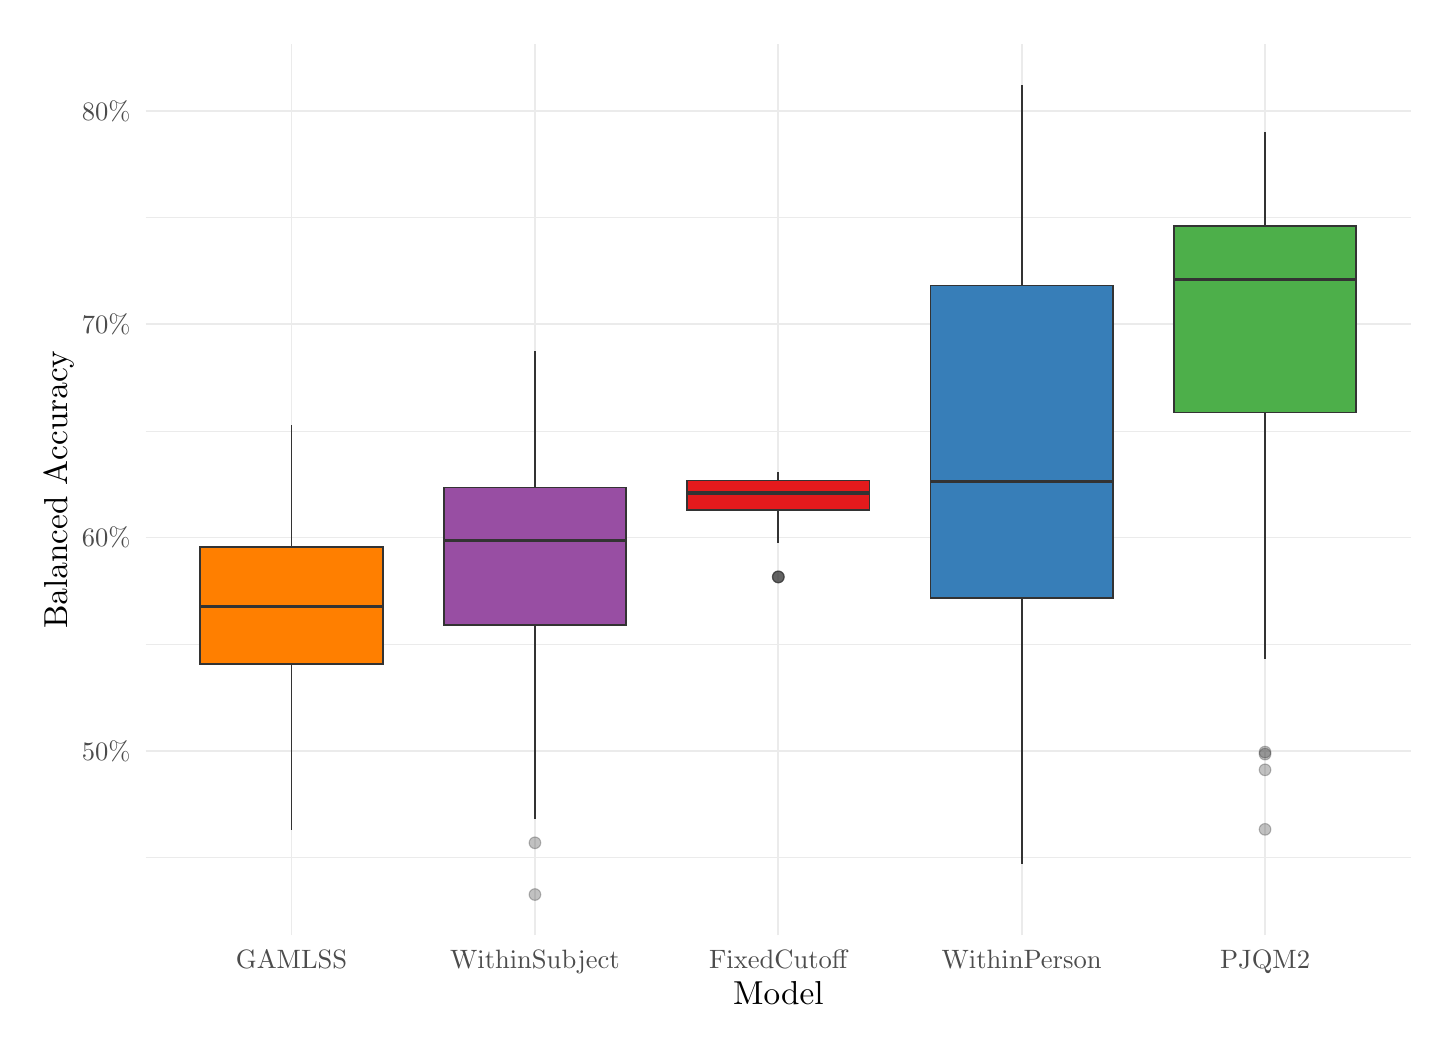
\begin{tikzpicture}[x=1pt,y=1pt]
\definecolor{fillColor}{RGB}{255,255,255}
\path[use as bounding box,fill=fillColor,fill opacity=0.00] (0,0) rectangle (505.89,361.35);
\begin{scope}
\path[clip] (  0.00,  0.00) rectangle (505.89,361.35);
\definecolor{fillColor}{RGB}{255,255,255}

\path[fill=fillColor] (  0.00,  0.00) rectangle (505.89,361.35);
\end{scope}
\begin{scope}
\path[clip] ( 42.59, 33.48) rectangle (499.89,355.35);
\definecolor{drawColor}{gray}{0.92}

\path[draw=drawColor,line width= 0.3pt,line join=round] ( 42.59, 61.47) --
	(499.89, 61.47);

\path[draw=drawColor,line width= 0.3pt,line join=round] ( 42.59,138.55) --
	(499.89,138.55);

\path[draw=drawColor,line width= 0.3pt,line join=round] ( 42.59,215.62) --
	(499.89,215.62);

\path[draw=drawColor,line width= 0.3pt,line join=round] ( 42.59,292.69) --
	(499.89,292.69);

\path[draw=drawColor,line width= 0.6pt,line join=round] ( 42.59,100.01) --
	(499.89,100.01);

\path[draw=drawColor,line width= 0.6pt,line join=round] ( 42.59,177.08) --
	(499.89,177.08);

\path[draw=drawColor,line width= 0.6pt,line join=round] ( 42.59,254.16) --
	(499.89,254.16);

\path[draw=drawColor,line width= 0.6pt,line join=round] ( 42.59,331.23) --
	(499.89,331.23);

\path[draw=drawColor,line width= 0.6pt,line join=round] ( 95.36, 33.48) --
	( 95.36,355.35);

\path[draw=drawColor,line width= 0.6pt,line join=round] (183.30, 33.48) --
	(183.30,355.35);

\path[draw=drawColor,line width= 0.6pt,line join=round] (271.24, 33.48) --
	(271.24,355.35);

\path[draw=drawColor,line width= 0.6pt,line join=round] (359.18, 33.48) --
	(359.18,355.35);

\path[draw=drawColor,line width= 0.6pt,line join=round] (447.12, 33.48) --
	(447.12,355.35);
\definecolor{drawColor}{gray}{0.20}

\path[draw=drawColor,line width= 0.6pt,line join=round] ( 95.36,173.70) -- ( 95.36,217.68);

\path[draw=drawColor,line width= 0.6pt,line join=round] ( 95.36,131.35) -- ( 95.36, 71.34);
\definecolor{fillColor}{RGB}{255,127,0}

\path[draw=drawColor,line width= 0.6pt,fill=fillColor] ( 62.38,173.70) --
	( 62.38,131.35) --
	(128.34,131.35) --
	(128.34,173.70) --
	( 62.38,173.70) --
	cycle;

\path[draw=drawColor,line width= 1.2pt] ( 62.38,152.11) -- (128.34,152.11);
\definecolor{drawColor}{RGB}{51,51,51}
\definecolor{fillColor}{RGB}{51,51,51}

\path[draw=drawColor,draw opacity=0.30,line width= 0.4pt,line join=round,line cap=round,fill=fillColor,fill opacity=0.30] (183.30, 66.80) circle (  2.11);

\path[draw=drawColor,draw opacity=0.30,line width= 0.4pt,line join=round,line cap=round,fill=fillColor,fill opacity=0.30] (183.30, 48.11) circle (  2.11);
\definecolor{drawColor}{gray}{0.20}

\path[draw=drawColor,line width= 0.6pt,line join=round] (183.30,195.21) -- (183.30,244.59);

\path[draw=drawColor,line width= 0.6pt,line join=round] (183.30,145.53) -- (183.30, 75.34);
\definecolor{fillColor}{RGB}{152,78,163}

\path[draw=drawColor,line width= 0.6pt,fill=fillColor] (150.32,195.21) --
	(150.32,145.53) --
	(216.28,145.53) --
	(216.28,195.21) --
	(150.32,195.21) --
	cycle;

\path[draw=drawColor,line width= 1.2pt] (150.32,176.07) -- (216.28,176.07);
\definecolor{drawColor}{RGB}{51,51,51}
\definecolor{fillColor}{RGB}{51,51,51}

\path[draw=drawColor,draw opacity=0.30,line width= 0.4pt,line join=round,line cap=round,fill=fillColor,fill opacity=0.30] (271.24,162.88) circle (  2.11);

\path[draw=drawColor,draw opacity=0.30,line width= 0.4pt,line join=round,line cap=round,fill=fillColor,fill opacity=0.30] (271.24,162.88) circle (  2.11);

\path[draw=drawColor,draw opacity=0.30,line width= 0.4pt,line join=round,line cap=round,fill=fillColor,fill opacity=0.30] (271.24,162.88) circle (  2.11);

\path[draw=drawColor,draw opacity=0.30,line width= 0.4pt,line join=round,line cap=round,fill=fillColor,fill opacity=0.30] (271.24,162.88) circle (  2.11);
\definecolor{drawColor}{gray}{0.20}

\path[draw=drawColor,line width= 0.6pt,line join=round] (271.24,197.67) -- (271.24,200.96);

\path[draw=drawColor,line width= 0.6pt,line join=round] (271.24,186.97) -- (271.24,175.19);
\definecolor{fillColor}{RGB}{228,26,28}

\path[draw=drawColor,line width= 0.6pt,fill=fillColor] (238.26,197.67) --
	(238.26,186.97) --
	(304.22,186.97) --
	(304.22,197.67) --
	(238.26,197.67) --
	cycle;

\path[draw=drawColor,line width= 1.2pt] (238.26,193.22) -- (304.22,193.22);

\path[draw=drawColor,line width= 0.6pt,line join=round] (359.18,268.23) -- (359.18,340.72);

\path[draw=drawColor,line width= 0.6pt,line join=round] (359.18,155.35) -- (359.18, 59.25);
\definecolor{fillColor}{RGB}{55,126,184}

\path[draw=drawColor,line width= 0.6pt,fill=fillColor] (326.21,268.23) --
	(326.21,155.35) --
	(392.16,155.35) --
	(392.16,268.23) --
	(326.21,268.23) --
	cycle;

\path[draw=drawColor,line width= 1.2pt] (326.21,197.43) -- (392.16,197.43);
\definecolor{drawColor}{RGB}{51,51,51}
\definecolor{fillColor}{RGB}{51,51,51}

\path[draw=drawColor,draw opacity=0.30,line width= 0.4pt,line join=round,line cap=round,fill=fillColor,fill opacity=0.30] (447.12, 71.66) circle (  2.11);

\path[draw=drawColor,draw opacity=0.30,line width= 0.4pt,line join=round,line cap=round,fill=fillColor,fill opacity=0.30] (447.12, 93.17) circle (  2.11);

\path[draw=drawColor,draw opacity=0.30,line width= 0.4pt,line join=round,line cap=round,fill=fillColor,fill opacity=0.30] (447.12, 98.85) circle (  2.11);

\path[draw=drawColor,draw opacity=0.30,line width= 0.4pt,line join=round,line cap=round,fill=fillColor,fill opacity=0.30] (447.12, 99.59) circle (  2.11);
\definecolor{drawColor}{gray}{0.20}

\path[draw=drawColor,line width= 0.6pt,line join=round] (447.12,289.62) -- (447.12,323.74);

\path[draw=drawColor,line width= 0.6pt,line join=round] (447.12,222.33) -- (447.12,133.28);
\definecolor{fillColor}{RGB}{77,175,74}

\path[draw=drawColor,line width= 0.6pt,fill=fillColor] (414.15,289.62) --
	(414.15,222.33) --
	(480.10,222.33) --
	(480.10,289.62) --
	(414.15,289.62) --
	cycle;

\path[draw=drawColor,line width= 1.2pt] (414.15,270.36) -- (480.10,270.36);
\end{scope}
\begin{scope}
\path[clip] (  0.00,  0.00) rectangle (505.89,361.35);
\definecolor{drawColor}{gray}{0.30}

\node[text=drawColor,anchor=base east,inner sep=0pt, outer sep=0pt, scale=  0.96] at ( 37.19, 96.70) {50\%};

\node[text=drawColor,anchor=base east,inner sep=0pt, outer sep=0pt, scale=  0.96] at ( 37.19,173.78) {60\%};

\node[text=drawColor,anchor=base east,inner sep=0pt, outer sep=0pt, scale=  0.96] at ( 37.19,250.85) {70\%};

\node[text=drawColor,anchor=base east,inner sep=0pt, outer sep=0pt, scale=  0.96] at ( 37.19,327.92) {80\%};
\end{scope}
\begin{scope}
\path[clip] (  0.00,  0.00) rectangle (505.89,361.35);
\definecolor{drawColor}{gray}{0.30}

\node[text=drawColor,anchor=base,inner sep=0pt, outer sep=0pt, scale=  0.96] at ( 95.36, 21.46) {GAMLSS};

\node[text=drawColor,anchor=base,inner sep=0pt, outer sep=0pt, scale=  0.96] at (183.30, 21.46) {WithinSubject};

\node[text=drawColor,anchor=base,inner sep=0pt, outer sep=0pt, scale=  0.96] at (271.24, 21.46) {FixedCutoff};

\node[text=drawColor,anchor=base,inner sep=0pt, outer sep=0pt, scale=  0.96] at (359.18, 21.46) {WithinPerson};

\node[text=drawColor,anchor=base,inner sep=0pt, outer sep=0pt, scale=  0.96] at (447.12, 21.46) {PJQM2};
\end{scope}
\begin{scope}
\path[clip] (  0.00,  0.00) rectangle (505.89,361.35);
\definecolor{drawColor}{RGB}{0,0,0}

\node[text=drawColor,anchor=base,inner sep=0pt, outer sep=0pt, scale=  1.20] at (271.24,  8.33) {Model};
\end{scope}
\begin{scope}
\path[clip] (  0.00,  0.00) rectangle (505.89,361.35);
\definecolor{drawColor}{RGB}{0,0,0}

\node[text=drawColor,rotate= 90.00,anchor=base,inner sep=0pt, outer sep=0pt, scale=  1.20] at ( 14.26,194.41) {Balanced Accuracy};
\end{scope}
\end{tikzpicture}
